% !TeX document-id = {acd94374-0a5a-4c39-a15c-8f2e56f0151a}
\documentclass[12pt,a4paper, listof=entryprefix, bibliography=totocnumbered,toc=listofnumbered,lof=listofnumbered]{scrartcl}

% WICHTIG!!!
% Pseudokommentar um pdflatex zu erlauben andere Programme zu nutzen z.B. gnuplot
% !TeX TXS-program:compile = txs:///pdflatex/[--shell-escape] 

\usepackage[ngerman]{babel}
\usepackage[utf8]{inputenc}
\usepackage{amsmath}
\usepackage{nccmath}
\usepackage{amsfonts}
\usepackage{amssymb}
\usepackage{graphicx}
\usepackage{fancyhdr}
\usepackage{tabularx}
\usepackage{geometry}
\usepackage{setspace}
\usepackage[right]{eurosym}
\usepackage[printonlyused]{acronym}
\usepackage{subfig}
\usepackage{floatflt}
\usepackage[usenames,dvipsnames]{color}
\usepackage{colortbl}
\usepackage{xcolor}
\usepackage{paralist}
\usepackage{array}
\usepackage{titlesec}
\usepackage{parskip}
\usepackage{picinpar}
\usepackage[pdfpagelabels=true]{hyperref}
\usepackage{listings}
\usepackage{csquotes}
\usepackage{url}
\usepackage{float}
\usepackage{pgfplots}
\usepackage{paralist}
\usepackage[nonumberlist, nogroupskip]{glossaries}

%-----------------------------------------------------------------------------------
% Bibilothek
%-----------------------------------------------------------------------------------
% Einbinden des BibLateX paketes mit Ausgabeeinstellungen
\usepackage[
style=alphabetic,          % Zitierstil
maxbibnames=50,            % alle Autorennamen anzeigen
maxcitenames=4,            % maximale Namen, die im Kürzel angezeigt werden
autocite=inline,           % regelt Aussehen für \autocite (inline=\parancite)
block=space,               % kleiner horizontaler Platz zwischen den Feldern
backref=true,              % Seiten anzeigen, auf denen die Referenz vorkommt
backrefstyle=three+,       % fasst Seiten zusammen, z.B. S. 2f, 6ff, 7-10
date=short,                % Datumsformat
backend = biber,           % Backnend für Aufbereitung
]{biblatex}

%Zusätzliche für Umbrüche für Kleinbuchstaben z.B. in URLs
\appto\UrlBreaks{\do\a\do\b\do\c\do\d\do\e\do\f\do\g\do\h\do\i\do\j
	\do\k\do\l\do\m\do\n\do\o\do\p\do\q\do\r\do\s\do\t\do\u\do\v\do\w
	\do\x\do\y\do\z}


\newcounter{verzeichnis}
\setcounter{verzeichnis}{1}

%Abstände der Einträge
\setlength{\bibitemsep}{1em}     % Abstand zwischen den Literaturangaben
\setlength{\bibhang}{2em}        % Einzug nach jeweils erster Zeile

% Kürzel soll vier Buchstaben der Autoren enthalten statt drei
\DeclareLabelalphaTemplate{
	\labelelement{
		\field[final]{shorthand}
		\field{label}
		\field[strwidth=4,strside=left,ifnames=1]{labelname}
		\field[strwidth=2,strside=left,ifnames=2]{labelname}
		\field[strwidth=1,strside=left]{labelname}
	}
	\labelelement{
		\field[strwidth=2,strside=right]{year}
	}
}

% Bibliothek der Quellen
\bibliography{bib}
\label{bib}

% --------------------------------------------------------------------------------
% Einstellung für Listings
% --------------------------------------------------------------------------------
\lstset{basicstyle=\footnotesize, captionpos=b, breaklines=true, showstringspaces=false, tabsize=2, frame=lines, numbers=left, numberstyle=\tiny, xleftmargin=2em, framexleftmargin=2em}
\makeatletter
\def\l@lstlisting#1#2{\@dottedtocline{1}{0em}{1em}{\hspace{1,5em} Lst. #1}{#2}}
\makeatother

% --------------------------------------------------------------------------------
% Seitenformate
% --------------------------------------------------------------------------------
%Seitenformat
\geometry{a4paper, top=27mm, left=30mm, right=20mm, bottom=32mm, headsep=12mm, footskip=12mm}

% --------------------------------------------------------------------------------
% Metainformationen
% --------------------------------------------------------------------------------
\hypersetup{unicode=false, pdftoolbar=true, pdfmenubar=true, pdffitwindow=false, pdfstartview={FitH},
	pdftitle={Vorlage},
	pdfauthor={Stefan Jung},
	pdfsubject={Abschlussarbeit},
	pdfcreator={\LaTeX\ with package \flqq hyperref\frqq},
	pdfproducer={pdfTeX \the\pdftexversion.\pdftexrevision},
	pdfkeywords={Vorlage},
	pdfnewwindow=true,
	colorlinks=true,linkcolor=black,citecolor=black,filecolor=magenta,urlcolor=black}
\pdfinfo{/CreationDate (D:20141024101000)}
\pgfplotsset{compat=1.11}

%-----------------------------------------------------------------------------------
% Abkürzungen AKRONYME HIER ERGÄNZEN
%-----------------------------------------------------------------------------------
\glssetwidest{OTHR}% Längste Abkürzung für eine korrekte Einrückung

\makenoidxglossaries %Leeres Verzeichnis erstellen

%Abkürzungen hinzufügen
\newacronym{LIP}{LIP}{Labor für Informationstechnik und Produktionslogistik}
\newacronym{OTH}{OTHR}{Ostbayerische Technische Hochschule Regensburg}
\newacronym{MRP}{MRP}{Material Requirements Planing}

\begin{document}
% --------------------------------------------------------------------------------
% Globale Formateinstellungen
% --------------------------------------------------------------------------------
\onehalfspacing
% Abstände Überschrift
\titlespacing{\section}{0pt}{42pt}{6pt}
\titlespacing{\subsection}{0pt}{12pt}{6pt}
\titlespacing{\subsubsection}{0pt}{12pt}{6pt}

% Kopf- und Fusszeile
\pagestyle{fancy}
\lhead{}\chead{}
\rhead{\thesection\space\contentsname}
\lhead{}\cfoot{}
\rfoot{\ \linebreak \thepage}
\renewcommand{\headrulewidth}{0.4pt}
\renewcommand{\footrulewidth}{0.4pt}

% Nummereriung
\renewcommand{\thesection}{\Roman{section}}
\renewcommand{\theHsection}{\Roman{section}}
\pagenumbering{Roman}

% eigene Farbdefinitionen
\definecolor{lip}{HTML}{3366FF}
\definecolor{grey}{HTML}{ABABAB}

% ---------------------------------------------------------------------------
% Titelseite
% ---------------------------------------------------------------------------
\thispagestyle{empty}

%LIP Schriftzug in eigener Farbe 
\textsf{\begin{minipage}{.69\textwidth}
	\large
	\textcolor{lip}{\textbf{Labor für Informationstechnik und\\Produktionslogistik (LIP)}} %Farbe setzten
	\small 
	\textbf{\\Verfahren, Strategien, Prozesse und IT-Systeme}
	\\Professor Dr.-Ing. Frank Herrmann
\end{minipage}
%Einbinden des OTH Logos mir rechtsbündiger Ausrichtung
\begin{minipage}{.29\textwidth}
	\begin{flushright}
		
\includegraphics[scale=.15]{Bilder/othlogo}\\
	\end{flushright}
\end{minipage}}
 
% Zeilenabstand
\onehalfspacing	

%Beschriftung der Titelseite
\begin{center}

	\vspace*{4cm} %4 cm Vorspann
	\Large
	\textbf{\LaTeX-Vorlage}\\ %Titel der Arbeit
	\large
	\textbf{für Fallstudien}\\ %Untertitel der Arbeit
		
	\vspace*{8cm} %8 cm Vorspann
	\normalsize
	\begin{center}
	Oktober 2014\\
	\textbf{Stefan Jung (B.Sc)} %Name des Autors
	
	\end{center}
\end{center}
\pagebreak

% ------------------------------------------------------------------------------
% Inhaltsverzeichnis
% ------------------------------------------------------------------------------
% Inhaltsverzeichnis
\singlespacing %Zeilenabsatnd reduzieren
\setcounter{section}{0}
\setcounter{page}{1}
\addcontentsline{toc}{section}{Inhaltsverzeichnis}%hinzufügen des Inhaltsverzeichnises selbst

\tableofcontents %Ausgabe des Inhaltsverzeichnisses
\pagebreak

% ------------------------------------------------------------------------------
% Setzen der Nummerierungen für Normaltext
% ------------------------------------------------------------------------------
\onehalfspacing %Zeilenabstand auf 1.5
\renewcommand{\thesection}{\arabic{section}} %Arabische Beschriftung für Absatznummern
\pagenumbering{arabic}  %Seitennummerrierung auf arabisch setzten
\setcounter{page}{1}	%Seitenzahl für Inhalt auf 1 setzten
\setcounter{section}{0}
% Kopfzeile mit aktuellem Hauptkapitel darstellen
\renewcommand{\sectionmark}[1]{\markright{#1}} %Section ausgeben
\renewcommand{\subsectionmark}[1]{}            %Subsection nicht ausgeben
\renewcommand{\subsubsectionmark}[1]{}         %Subsubsection nicht ausgeben
\rhead{\rightmark}                             %Ausgabe Rechtsbündig

%------------------------------------------------------------------------------
%	Installation
%------------------------------------------------------------------------------
\section{Installation}
\label{ch:instalaltion}
In diesem kapitel werden die benötigten Komponenten genannt.

\subsection{TeX Live}
\label{ch:texlive}
Um ein \LaTeX-Dokument erstellen zu können muss eine aktuelle Version von TeX Live installiert werden. Zu finden ist der Windowsinstaller unter \url{https://www.tug.org/texlive/acquire-netinstall.html}. Für eine korrekte Installation ist den dort hinterlegten Installationsanweisungen zu folgen.

TeX Live ist derzeit die umfangreichste \LaTeX-Distribution und beinhaltet alle gängigen Pakete und Anwendungen, daher ist zu beachten, dass ca. 4 GB Festplattenspeicher vorhanden sind.

\subsection{TexStudio}
\label{ch:texstudio}
Ergänzend zu TeX Live ist eine Editor notwendig. Empfohlen wird TexStudio in aktueller Version, zu finden unter \url{http://texstudio.sourceforge.net/}.

TexStudio bietet als Umgebung Reiter zu unterschiedliche Themengebieten von \LaTeX und die am häufigsten benötigten Befehle, die im folgenden Dokument zum Teil vorgestellt werden. 

\subsection{Gnuplot}
\label{ch:gnuplot}
Um Funktionen plotten zu können muss das Programm gnuplot auf dem PC installiert werden. Das Programm kann unter \url{http://sourceforge.net/projects/gnuplot/files/gnuplot/} gedownloadet werden. 

Für die Verwendung von gnuplot is es notwendig die Umgebungsvariable PATH um den Pfad der gnuplot.exe zu ergänzen. Eine Anleitung dazu kann \url{http://www.proggen.org/doku.php?id=windows:faq:envvars} entnommen werden.

\subsection{Citavi}
\label{ch:citavi}
Um die verwendete Literatur ordentlich Verwalten zu können wird Citavi empfohlen, welches der Hochschule als Campuslizenz zur Verfügung steht.
Die Downloaddatei ist unter \url{http://www.citavi.com/de/download.html} zu finden.\\
Die benötigte Lizenzdatein ist unter \url{http://www.citavi.com/license/start/email-email-de.php?n=Hochschule+Regensburg+-+Citavi+Team} zu beantragen.

Citavi bietet die Möglichkeit Literatur in einem Projekt zu organisieren und in einer von \LaTeX nutzbaren Form zu exportieren. Um sicherzustellen, dass die Exporte im korrekten Format für \LaTeX angefertigt werden müssen unter Extras$\rightarrow$Optionen folgende Einstellungen vorgenommen werden:

\begin{figure}[H]
	\centering
	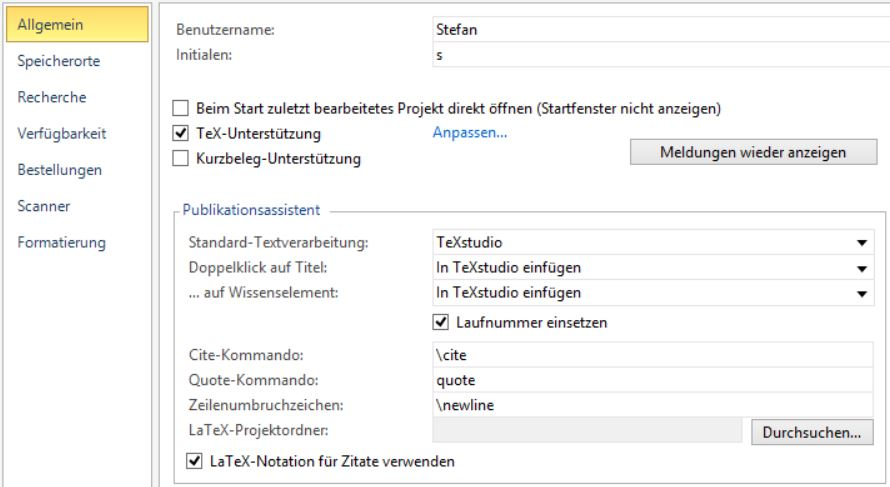
\includegraphics[width=0.8\linewidth]{Bilder/citavi.jpg} 
	\captionof{figure}[Citavi Einstellungen]{Citavi Einstellungen für Bibliotheken}
	\label{fig:citavi}
\end{figure}

Danach können die Quellen wie folgt exportiert werden:
\begin{compactitem}
	\item Wählen Sie im Programmteil Literaturverwaltung aus dem Menü Datei den Befehl Exportieren…
	\item Entscheiden Sie sich, ob Sie alle Titel, nur die markierten Titel oder die Titel der aktuellen Auswahl exportieren möchten.
	\item Entscheiden Sie sich für das BibLaTeX-Format.
	\item Klicken Sie auf die Schaltfläche Durchsuchen, um einen Ordner auf Ihrem Computer auszuwählen, in dem die Datei gespeichert werden soll.
	\item Klicken Sie auf die Schaltfläche Fertigstellen.
	\item Citavi meldet Ihnen den abgeschlossenen Export mit dem Dialogfeld »Export erfolgreich abgeschlossen«.
\end{compactitem}

Um die exportierte Bibliothek in \LaTeX nutzen zu können muss das Bibliotheksprogramm auf Biber eingestellt werden. Dies erfolgt unter Optionen$\rightarrow$TeXstudio konfigurieren$\rightarrow$Erzeugen wie folgt vorzunehmen:
\begin{figure}[H]
	\centering
	\includegraphics[width=0.8\linewidth]{Bilder/biber.jpg} 
	\captionof{figure}[Citavi Einstellungen]{Citavi Einstellungen für Bibliotheken}
	\label{fig:citavi}
\end{figure}

Zusätzlich muss die Bibliographieart unter Bibliographie$\rightarrow$Bibliographieart auf BibLaTeX gestellt werden.

Die exportierte Bibliothek kann für das Quellenverzeichnis (erläutert in \ref{ch:quellen}) über den Befehl \textit{\textbackslash biblography} im Dokumentkopf eingetragen werden. Daraus erstellt \LaTeX automatisch das Quellenverzeichnis.

\pagebreak

%------------------------------------------------------------------------------
%	Fließtext
%------------------------------------------------------------------------------
\section{Flie{\ss}text}
\label{ch:fliesstext}
Dieses Kapitel enthält Beispiele und Anleitungen für das Erstellen und Formatieren von Fließtext.

%Beschreibung wie in LaTeX gegliedert wird
\subsection{Gliederung}
\label{ch:Gliederung}
Die Gliederung in \LaTeX erfolgt über das setzen von Sektionen und Paragraphen. Die ersten drei Gliederungsebenen werden mit den Befehlen \textit{\textbackslash section, \textbackslash subsection} und \textit{\textbackslash subsubsection} gebildet und werden auch in die Gliederung übernommen. Zwei zusätzliche Ebenen können mit \textit{\textbackslash paragraph} und \textit{\textbackslash subparagraph} gebildet werden. \LaTeX organisiert die Formatierung und Nummerierung automatisch.

Vor jeder neuen \textit{section} muss mit \textit{pagebreak} ein Seitenumbruch erzeugt werden. So werden die einzelnen Kapitel getrennt.

%Beschreibung der zu verwendenden Schriftgrößen
\subsection{Schrift}
\label{ch:schrift}
In \LaTeX gibt es keine eigenen Schriftarten oder Schriftgrößen wie sie aus Word bekannt sind. Es existiert lediglich die hier verwendete Schriftart, die mit Hilfe von Befehlen formatiert werden kann. Im Umfeld der Fallstudiendokumentation sind nachfolgende Schriftgrößen mit ihren ungefähren Entsprechungen in MS Word dargestellt. 

\begin{table}[H]
	\centering
	\begin{tabular}{|l|l|l|l|}
	\hline  \textbackslash Large& \textbackslash large & \textbackslash normalsize & \textbackslash small \\ 
	\hline  17pt & 14pt & 12pt & 11pt   \\ 
	\hline 
	\end{tabular} 
	\caption{Schriftgrößen} %Hinzufügen einer Tabellenbeschriftung
	\label{tab:schriftgroessen}
	
\end{table}

\subsection{Absätze}
\label{ch:absaetze}
Absätze werden über eine Leerzeile im Text gebildet. Normale Umbrüche können mit \textit{\textbackslash\textbackslash} erzeugt werden, allerdings wird dabei kein Abstand gebildet. Für diese Funktionalität muss das Paket \textit{parskip} eingebunden werden. Es folgt ein Beispiel:

Lorem ipsum dolor sit amet, consetetur sadipscing elitr, sed diam nonumy eirmod tempor invidunt ut labore et dolore magna aliquyam erat, sed diam voluptua.

%Neuer Absatz da eine Leerzeile vorranging
Neue Absatz. At vero eos et accusam et justo duo dolores et ea rebum. Stet clita kasd gubergren, no sea takimata sanctus est Lorem ipsum dolor sit amet. \\ %Neue Teile da hier mit \\ umgebrochen wird
Neuer Zeile. Lorem ipsum dolor sit amet, consetetur sadipscing elitr, sed diam nonumy eirmod tempor invidunt ut labore et dolore magna aliquyam erat, sed diam voluptua. 

\subsection{Hervorhebung}
\label{ch:hervorhebung}
Um Wörter ein einem Text hervorzuheben wird der befehlt \textit{\textbackslash emph} verwendet.
\\ z.B.: Hier wird ein \emph{Wort} hervorgehoben.

Um Befehle oder einzelne Syntaxelemente wie Methodennamen in einen Fliesstext einzubinden wird der Befehlt \textit{\textbackslash textit} verwendet. 
\\z.B.: Jede nichtabstarakte Klasse besitzt eine Methode \textit{constructor()}.

\subsection{Sonderzeichen}
\label{ch:zeichen}

In \LaTeX sind viele Sonderzeichen bereits vorbelegt und müssen daher über eigene Befehle ausgegeben werden. Ergänzt wird die Liste durch eine Vielzahl an mathematischer Sonderzeichen. Die wichtigsten Sonderzeichen können unter \url{http://de.wikibooks.org/wiki/LaTeX-Kompendium:_Sonderzeichen} eingesehen werden.


% !TEX root = ../Vorlage.tex

\subsection{Modularisierung}
\LaTeX bietet die Möglichkeit der Modularisierung. Das heißt, dass Kapitel als Includes zu einem gesamten Dokument zusammengeführt werden können. Dabei werden alle Einstellungen in einem Hauptdokument vorgenommen und die Inhalte des Dokuments über den Befehl $\backslash include$ eingebunden. Die Includes definieren nur Dokumenteninhalt und verweisen auf ihr Hauptdokument. Als Beispiel wird dieser Punkt als Include eingebunden. Es muss dabei beachtet werden, dass nach jedem Include ein Seitenumbruch erfolgt. Daher wird die Verwendung von Includes nur für Sections empfohlen.




%------------------------------------------------------------------------------
%	Objekte
%------------------------------------------------------------------------------
\section{Objekte}
\label{ch:objekte}
Dieses Kapitel enthält Beispiele zum Einfügen von Abbildungen, Tabellen, etc..
 
\subsection{Auflistung}

Für Auflistungen wird die \textit{compactitem}-Umgebung genutzt, wodurch der Zeilenabstand zwischen den Punkten verringert wird. Beispielcode kann dem Quelltext zu diesem Punkt entnommen werden.

% Einfache Aufzählung
\begin{compactitem}
	\item Nur
	\item ein
	\item Beispiel
	% Unterpunkte
	\begin{compactitem}
		\item mit
		\item Einrückung
	\end{compactitem}
\end{compactitem}

\subsection{Referenzen}
\label{ch:referenz}
Um auf ein Bild, eine Tabelle, ein Kapitel, oder anderen Inhalten eine \LaTeX-Dokuments verweisen zu können, ist es notwendig das gewünschte Objekt mit einem Label zu versehen. Dies geschieht durch den Befehlt \textit{\textbackslash label} nach dem Objekt. Um die Referenzen besser verwenden zu können sind diese, entsprechend ihres Ziels, mit einem Präfix zu versehen. Daraus ergibt sich der Aufbau \textit{\textbackslash label\{\textless prefix\textgreater:\textless name\textgreater\}}. Dabei ist zu beachten, dass in der Labelbezeichnung außer des Präfixes keine Sonderzeichen oder Umlaute verwendet werden dürfen.

% Liste mit Präfixen für Labelbeschriftung
\begin{compactitem}
	\item Bild fig:
	\item Tabelle tab:
	\item Kapitel ch:
	\item Code-Listing lst:
	\item Anhang app:
	\item Zitat eq:
\end{compactitem}

% Wie kann ich auf ein Label refernezieren?
Für die Referenzierung auf ein Label im Text wird der Befehl \textit{\textbackslash ref} durchgeführt.\\
z.B. Verweis auf Kapitel der Referenzen in Kapitel \ref{ch:referenz}

% Wie kann ich auf die Seite eines Labels refenzieren?
Um auf die Seite eines Objekts zu referenzieren wird der Befehl \textit{\textbackslash refpage} verwendet.\\
z.B. Dieses Kapitel befindet sich auf Seite \pageref{ch:referenz}

%Beschreibung wie Fussnoten eingefügt werden
\subsection{Fussnoten}
\label{ch:fussnoten}
Anmerkungen und Fußnoten sollen vermieden werden. Wenn die Nutzung unumgänglich ist (z.B. Hinweise auf Fehler in der Originalquelle), werden die Anmerkungen mit hochgestellten Ziffern durchnummeriert. Fussnoten werden über den Befehl \textit{\textbackslash footmark} in den Text eingebunden und mit \textit{\textbackslash footnotetext} die entsprechende Quelle geschaffen. 

% Hier wird der Verweis gesetzt
z.B. eine Fussnote zu obigem Bild \footnotemark 
% Das hier steht in der Fusszeile
\footnotetext{Quelle: \url{http://www.osgi.org/Technology/WhatIsOSGi}}

\subsection{Bilder}
\label{ch:bilder}
Grafiken, Fotos oder Diagramme sollten drucktauglich sein und in der wiederzugebenden Größe in der Ausarbeitung an der gewünschten Position eingefügt werden. Grafiken sollen in Visio erstellt und als PDFs eingebunden werden. Visio kann über eine Studentenlizenz unter \url{https://www.oth-regensburg.de/dreamspark/index.php?action=signin} bezogen werden.

Die Visio-Datein müssen für ihre Verwendung in \LaTeX um ihren Rand bereinigt werden. Dazu müssen unter Datei$\rightarrow$Optionen$\rightarrow$Menüband anpassen die Entwicklertools aktiviert werden. Anschließend müssen im Reiter Entwicklertools unter Menüpunkt Shapesheet anzeigen$\rightarrow$Zeichenblatt die Seitenränder der Druckeinstellungen auf 0mm gesetzt werden (vgl. Abbildung \ref{fig:visio}).

\begin{figure}[H]
	\centering
	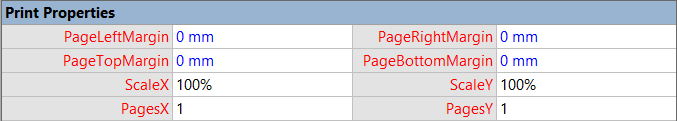
\includegraphics[width=0.8\linewidth]{Bilder/Visio.png} 
	\captionof{figure}[Visio]{Seitenränder in Visio auf 0 setzten}
	\label{fig:visio}
\end{figure}

Ein Beispiel kann den \LaTeX-Quelltext entnommen werden. Es ist zu beachten, dass alle verwendeten Bilder im Ordner \emph{Bilder} des Dokumentenverzeichnisses abgelegt werden und mit diesem Pfad eingebunden werden müssen.

%Einbinden eines Bildes aus dem Ordner Bilder in der Dokumentenorderstruktur. Das Bild wir auf 70 % der gesamten Zeilenbreite skaliert. Mit captionof{} wird dem Bild eine Abbildungsbeschriftung hinzugefügt. Mit \centering wird das Bild zentriert. Mit \label{key} kann auf das Bild referenziert werden.
\begin{figure}[H]
	\centering
	
\includegraphics[width=0.5\linewidth]{Bilder/othlogo} 
	\captionof{figure}[OTHR-Logo]{OTH Regensburg-Logo}
	\label{fig:osgi}
\end{figure}

\subsection{Tabellen}
\label{ch_tabellen}
In diesem Abschnitt wird eine Tabelle (siehe Tabelle \ref{tab:beispiel}) dargestellt. Wie eine Tabelle erstellt wird ist dem \LaTeX-Quellcode zu entnehmen. Nützliche Hinweise für die Erstellung von Tabellen sind Unter \url{http://en.wikibooks.org/wiki/LaTeX/Tables} zu finden. Die Tabelle selbst ist zentriert auszurichten.

\begin{table}[H]	%Beginn der Tabelle; [H] setzt die Tabelle an die aktuelle Cursorposition
	\centering		%Tabelle wird zentriert
	\begin{tabularx}{\linewidth}{|X|X|X|X|}  
	\hline %horizontale Trennlinie
	\multicolumn{4}{|l|}{Erzeugnis Tisch}\\ \hline 
	\hline %horizontale Trennlinie
	\rowcolor{grey} Position & Sachnummer & Menge & Bezeichnung \\ \hline 
	1 &	Tischplatte & 1 & Einzelteil       \\ %Spalteninhalt
	2 &	Befestigungselem. & 8 & Einzelteil \\ %Spalteninhalt
	3 &	Tischbein &	4 &	Baugruppe          \\ %Spalteninhalt
	\hline %horizontale Trennlinie
	\end{tabularx}
	\caption{Beispieltabelle} %Hinzufügen einer Tabellenbeschriftung
	\label{tab:beispiel}
\end{table}


\subsection{Pseudocode und Quelltext}
\label{ch:code}
Zuletzt ein Beispiel für ein Listing, in dem Quellcode eingebunden werden kann, siehe Listing \ref{lst:code}. Bei der Wiedergabe von Pseudocode sind die Bestimmungen für Pseudocode vermerkt in
\textbackslash\textbackslash rfhinffs1\textbackslash labor\textbackslash LO \textbackslash LIP\textbackslash Gemeinsames\textbackslash Organisation\textbackslash Dokumentations-richtlinie\textbackslash zu beachten.

% Zusätzlich eine Zeile Abstand
\vspace{1em}
% Beschriftung und Label wird direkt nach dem Beginn des Listings angegeben
%Zwischen begin und end des listings wird alles als Code formatiert
\begin{lstlisting}[caption= Beispielprogramm, label=lst:code]
int ledPin = 13;
void setup() {
    pinMode(ledPin, OUTPUT);
}
void loop() {
    digitalWrite(ledPin, HIGH);
    delay(500);
    digitalWrite(ledPin, LOW);
    delay(500);
}
\end{lstlisting}

\subsection{Diagramme}
\label{ch:diagramm}
Diagramme sollen wie Bilder in Visio erstellt und auch wie dort beschrieben eingebunden werden.

Eine zusätzliche Möglichkeit für komplexe Diagrammen ist die  Verwendung von \textit{gnuplot} und \textit{TikZ}. Dieses Programm stellt umfassende Funktionen zur Erstellung unterschiedlicher Funktionen zur Verfügung. Gerade bei sehr komplexen Diagrammen ist die Einarbeitung aber segr aufwendig.

Eine ausführliche Dokumentation über die Verwendung von \textit{TikZ} ist unter \url{http://ctan.mirrors.hoobly.com/graphics/pgf/base/doc/pgfmanual.pdf} zu finden.

% Zentrale Ausrichtung der Diagramme
\begin{center} 
\begin{tikzpicture}[domain=0:4]
\draw[very thin,color=gray] (-0.1,-1.0) grid(3.9,3.9);
\draw[->] (-0.2,0) -- (4.2,0) node[right] {$x$};
\draw[->] (0,-1.2) -- (0,4.2) node[above] {	$f(x)$};
\draw[color=red] plot[id=x] function{x} node[right] {$f(x)=x$};
\draw[color=blue] plot[id=sin] function{sin	(x)} node[right] {$f(x)=\sin$};
\draw[color=orange] plot[id=exp] function{0.05*exp(x)} node[right] {$f(x)=\frac{1}{20}e^x$};
\end{tikzpicture} 
\label{fig:diagramm}
\captionof{figure}[Diagramm]{Diagramm mit drei Funktionen}
\end{center}

\subsection{Formeln}
\label{ch:Formeln}
Formeln werden in einem abgesetzten Mathematikmodus erstellt. Die am häufigst verwendeten Formeln werden durch TexStudio im Reiter Mathe bereitgestellt. Ein Beispiel ist dem Quellcode zu entnehmen. Bei der Erstellung von Formeln ist unbedingt auf die korrekte Notation und Bezeichnung von Variablen zu achten. Eine Übersicht über viele Befehele ist unter \url{http://www-astro.physik.tu-berlin.de/files/Uebung/Dokumentationen/mathe_in_latex2e.pdf} zu finden.

% Formel linksbündig mit 1.25 cm Abstand
% Die Formlen werden anhand des ersten Zeichens nach dem & ausgerichtet
\begin{fleqn}[1.25cm]
\begin{align*}
	Y &= \sum_{i=1}^{n} x_{i} \\
	Ax &= \sum_{i=1}^{n} x_{i}
\end{align*}
\end{fleqn}

\subsection{Quellen}
\label{ch:quellen}
Die Quellen befinden sich in der Datei \textit{bib.bib}. Ein Buch- und eine Online-Quelle sind beispielhaft eingefügt. Für die Erstellung des Literaturverzeichnis wird BibLaTeX mit dem Backend Biber verwendet. Die Einstellungen für die Formatierung sind im Dokumentenkopf hinterlegt.

Um eine Quelle im Text zu nennen wird der Befehl \textit{\textbackslash cite} und der eindeutigen ID der Quelle wiedergegeben. \cite{Herrmann.2009}

Hinweis: Es kann sein, dass Änderungen im Quellenverzeichnis nicht übernommen werden, oder Fehler produzieren. Dann ist es sinnvoll alle Dateien des \LaTeX-Dokuments außer der Bibliothek, dem Bilderordner und das \LaTeX-File zu löschen und durch erneutes Speichern der Datei neu anzulegen.

\subsection{Abkürzungen}
\label{ch:abkuerzung}
Abkürzungen werden im  Kopfbereich erstellt. Neue Abkürzungen werden mit dem Befehl
\textit{\textbackslash newacronym\{\textless ID\textgreater\}\{\textless Abkürzung\textgreater\}\{\textless Langtext\textgreater\}} erstellt. Mit diesem Befehl werden Abkürzungen zur dokumenteigenen Abkürzungsbibliothek hinzugefügt werden. Jedes Element in dieser Bibliothek können über \textit{\textbackslash gls} und den eindeutigen Index ausgegeben werden. Dabei wird bei erster Verwendung Kurz- und Langform und im weiteren Verlauf nur noch die Kurzform ausgegeben. Hier ein Beispiel:

%Beispiel für die Verwendung von Abkürzungen
Für die Produktionsplanung ist ein \gls{MRP} von wichtiger Bedeutung. Für die Durchführung von \gls{MRP} stellt das Labor ein Tool zu Verfügung. 

Die Ausgabe der Verzeichnisses erfolgt automatisch und alphabetisch sortiert am Ende des Dokuments. Es ist zu beachten, dass das Abkürzungsverzeichnis erst nach zweimaligem Kompilieren vollständig angezeigt wird, da erst die Bibliothek erstellt und danach ausgelesen werden muss.

\subsection{Verzeichnisse}
\label{ch:verzeichnisse}
Bei korrekter Verwendung der Gliederungselemente (\textit{section}) und Objektbeschriftungen werden die Verzeichnisse wie Gliederung, Abbildungs-, Listing- und Tabellenverzeichnis automatisch erstellt.

\pagebreak

% ----------------------------------------------------------------------------------
% Anleitung wie eine Fallstudie aufgebaut ist
% ----------------------------------------------------------------------------------
\section{Einleitung}
\label{ch:einleitung}
In der Einleitung wird das Thema der Arbeit erläutert (z.B. Betrachtung der Durchlaufterminierung im \gls{MRP})

Daraus ist die Fragestellung, die mit der Fallstudie bearbeitet wird, abzuleiten und zu begründen (z.B. Wie wirkt sich die Vorlaufzeit auf die Berechnung der Durchlaufterminierung aus?)

\subsection{Rahmen}
\label{ch:rahmen}
Der Rahmen, indem die Fallstudie stattfindet, wird aufgezeigt (z.B.: Die Fallstudie entstand im Rahmen des Projektstudiums an der \gls{OTH} im \gls{LIP}). Damit wird der Umfang der erbrachten Arbeitszeit festgelegt und kann mit anderen, themenverwandten Fallstudien verglichen werden.

\subsection{Voraussetzungen}
\label{ch:vorraussetzungen}
Die Voraussetzungen beschreiben das notwendige Arbeitsumfeld. Dazu gehören verwendete Werkzeuge mit Versionsständen, eventuell verwendete Vorlagen etc. (z.B. Für die Bearbeitung der Fallstudien wurde das laboreigene MRP-Werkzeug in Version 1.1.6 verwendet. Als Vorlage für die Fallstudie dient eine Ausarbeitung aus \cite{Herrmann.2009} S. 271 ff..)

\subsection{Aufbau der Arbeit}
\label{ch:Aufbau}
Der Aufbau der Fallstudie (roter Faden) wird erläutert.

\pagebreak

\section{Theorieteil}
Erläutern Sie in diesem Kapitel die für ihre Fallstudie relevanten
Begriffe (z.B. Fachbegriffe, Bezeichnungen,...), Methoden und theoretischen Grundlagen.


Achten Sie möglichst darauf, dass dieser letzte Aspekt nicht durch eine ausführliche Beschreibung der einzelnen Punkte zu viel Raum einnimmt. Es sollen lediglich die wichtigen theoretischen Konzepte genannt und grob beschrieben werden.
Begriffe sollten jeweils definiert und kurz erläutert werden. Es muss deutlich werden, welche Theorien sie hier zu Grunde legen, darum ist es wichtig, die Aussagen mit Literaturquellen zu belegen.

Bei einer \gls{MRP}-Fallstudie kann beispielweise der allgemeine zweck eines \gls{MRP} aufgezeigt werden. Für die Betrachtung der Durchlaufterminierung ist deren Berechnungsweise zu nennen usw.

\pagebreak

\section{Praxisteil}
\label{ch:praxis}
In diesem Kapitel werden die durchgeführten Arbeiten schrittweise erläutert. Dabei ist zu beachten, dass die Beschreibung so aufgebaut sein soll, dass die Fallstudie unter Beachtung der Voraussetzungen von jedem Leser selbst umsetzbar ist.

\subsection{Beschreibung der Fallstudie}
\label{ch:beschreibung}
Hier wird die Ausgangsbasis der Fallstudie beschrieben. In der Regel existiert eine Fallstudie nicht einfach, sondern entsteht aus einem konstruierten Fall. 

Dieser Fall soll in seinem Aufbau wiedergegeben werden z.B. in einer \gls{MRP}-Fallstudie bildet eine Produktstückliste mit Bedarfen, Vorlaufzeiten und weiteren Parametern die Grundlage für Berechnungen. Diese Werte müssen demnach genannt und erläutert werden. Konkret heißt das für ein \gls{MRP}:

\begin{compactitem}
	\item Darstellen des Gozintogrpahen
	\item Aufzeigen von Bedarfen
	\item Erklärung für die Wahl bestimmter Werte wie z.B. Vorlaufzeiten
	\item Begründung für gewählte Verfahren
	\item ...
\end{compactitem}


\subsection{Inhaltliche Beschreibung}
\label{ch:inhalt}
Hier werden die durchgeführten Schritte der Fallstudie betrachtet. Dies umfasst das Erstellen des Falls, die Durchführung der Berechnungen, die Analyse der Berechnungen usw. Je nach Umfang der Arbeit ist hier eine sinnvolle Untergliederung angebracht.

\pagebreak

\section{Ergebnisse}
\label{ch:ergebnisse}
In Bezug auf die Fragestellung werden wichtige Aspekte der Beobachtung benannt (Querverweis auf einzelne Gliederungspunkte). Diese Aspekte müssen hier reflektiert werden, wobei Praxis und Theorie aufeinander bezogen werden.

Es sollen Erkenntnisse zur Fragestellung dargestellt werden, wobei diese nicht explizit beantwortet werden muss.
\pagebreak

%-------------------------------------------------------------------------------------
% Verzeichnisse %-------------------------------------------------------------------------------------
	\rhead{Verzeichnisse} %Kopftextbeschriftung

	\stepcounter{section}
	\phantomsection \label{Verzeichnisse}
	\addcontentsline{toc}{section}{Verzeichnisse} %Ohne Nummer ins Inhaltsverzeichnis
	\renewcommand{\thesection}{\Roman{verzeichnis}}
	\section*{Verzeichnisse}
	% Literaturverzeichnis
	\rhead{Verzeichnisse}
	\renewcommand{\refname}{Literaturverzeichnis}
	\printbibliography
	\pagebreak
	
	% Abbildungsverzeichnis
	\stepcounter{verzeichnis}
	\listoffigures
	\pagebreak
	
	% Tabellenverzeichnis
	\stepcounter{verzeichnis}
	\listoftables
	\pagebreak
	
	% Abkürzungen
	\stepcounter{verzeichnis}
	\section{Abkürzungsverzeichnis}
	\vspace{-6em} % Abstand analog der anderen Verzeichnisse reduzieren
	\printnoidxglossary[type=\acronymtype,style=alttree,title=,toctitle=] %automatischen Titel und Gliederungsbeschriftung unterdrücken - sonst steht da Glossarie
	\newpage

% ---------------------------------------------------------------------------------
% Anhang
% ---------------------------------------------------------------------------------
\pagenumbering{Roman} %Seitennummerierung auf Romanisch stellen
\setcounter{page}{1}  %Seitenzähler initialisieren
\rhead{Anhang}        %Kopftextbeschriftung
\begin{appendix}
	\phantomsection \label{Anhang}
	\section*{Anhang}\addcontentsline{toc}{section}{Anhang} %Anhang ohne Nummer
	\renewcommand{\thesection}{\Roman{section}}
	
	\setcounter{section}{0} %Counter für Nummerirung der Anhänge initalisieren
	\section{GUI}
	\label{app:gui}
	Ein toller Anhang.
	
	\section{Screenshot}
	\label{app:screenshot}
	Zweiter Anhang.
\end{appendix}

\end{document}
